% !TeX root = IoTStudy.tex
% !TeX encoding = UTF-8
% !TeX spellcheck = en_US


\begin{frame}{Basic}

	IoT is a huge field to study we need a mind map to help us to study it. But...
	\begin{alertblock}{What is IoT?}
		IoT is Internet of Things
	\end{alertblock}
	IoT started by monitoring a vending machine (coffee maker) to a computer to known if it was worth going to the room where the machine was\footnote{In other words if it was empty $\rightarrow$ don't go}.
\end{frame}

\begin{frame}{IoT Today}
	Today IoT can be defined as
	\begin{itemize}
		\item Evolution of M2M (Machine to Machine)
		\item A new Paradigm on design
		\item Democratization of M2M
		\item Distributed Computing, as it's maximum exponent
		\item Service Oriented ``Products''
	\end{itemize}
\end{frame}
\begin{frame}{Also}
	But also
	\begin{columns}
		\begin{column}{0.45\textwidth}
			\begin{block}{Synergies with:}
				\begin{itemize}
					\item Cloud Computing
					\item Machine Learning
					\item People
					\item Computer vision
					\item Augmented Reality
					\item Safety
				\end{itemize}
			\end{block}
		\end{column}
		\begin{column}{0.45\textwidth}
			\begin{block}{Has Cons:}
				\begin{itemize}
					\item Commercial Bluff
					\item Loss of service $\rightarrow$ bricks
					\item It is M2M, but for all
					\item Security issues
					\item Energy Consumption
					\item Extra network usage
				\end{itemize}
			\end{block}
		\end{column}
	\end{columns}
\end{frame}
\section{Initial MindMap}
\begin{frame}{Initial Map}
	\tikzset{
		treenode/.style = {shape=rectangle, rounded corners,
				draw, align=center,
				top color=white, bottom color=blue!20,
				font=\ttfamily\normalsize},
		root/.style     = {treenode, font=\Large, bottom color=red!30},
		def/.style      = {treenode, bottom color=green!20},
		syn/.style     = {treenode, bottom color=yellow!30},
		dummy/.style    = {circle,draw}
	}
	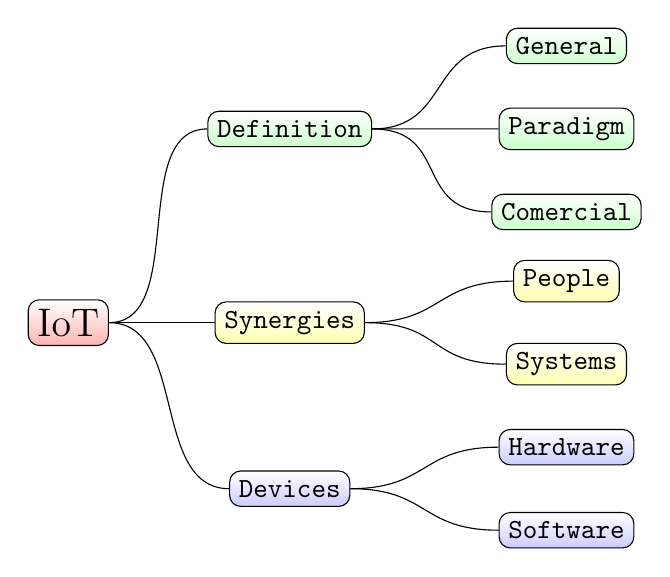
\begin{tikzpicture}
		[grow   = right,
			level distance          = 9em,
			edge from parent path= {(\tikzparentnode.east) .. controls +(1,0) and +(-1,0)  .. (\tikzchildnode.west)},
			every node/.style       = {font=\footnotesize},
			sloped,
			level 1/.style = { level distance = 8em, sibling distance = -6em},
			level 2/.style = {level distance   = 10em, sibling distance = -3em},
		]
		\node [root] {IoT}
		child { node [def, yshift=1em] {Definition}
				% edge from parent node [below] {single-line?} 
				child { node[def] {General} }
				child { node[def] {Paradigm} }
				child { node[def] {Comercial} }
			}
		child { node[syn] {Synergies}
				child { node[syn] {People} }
				child { node[syn] {Systems}}
			}
		child { node[treenode] {Devices}
				child { node[treenode] {Hardware} }
				child { node[treenode] {Software} }
			}
		;
	\end{tikzpicture}
\end{frame}
\begin{frame}{Definition}
	The study of the IoT definition should address the three main aspects or points of view relative to IoT
	\begin{columns}
		\begin{column}{0.45 \textwidth}
			\tikzset{
				treenode/.style = {shape=rectangle, rounded corners,
						draw, align=center,
						top color=white, bottom color=blue!20,
						font=\ttfamily\normalsize},
				root/.style     = {treenode, font=\Large, bottom color=red!30},
				def/.style      = {treenode, bottom color=green!20},
				syn/.style     = {treenode, bottom color=yellow!30},
				dummy/.style    = {circle,draw}
			}

			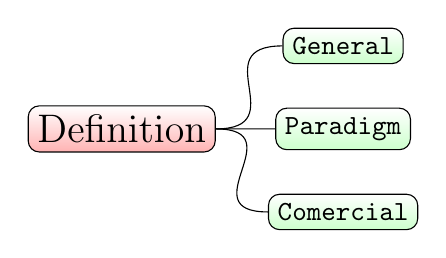
\begin{tikzpicture}
				[grow   = right,
					level distance          = 9em,
					edge from parent path= {(\tikzparentnode.east) .. controls +(1,0) and +(-1,0)  .. (\tikzchildnode.west)},
					every node/.style       = {font=\footnotesize},
					sloped,
					level 1/.style = { level distance = 8em, sibling distance = -3em},
					level 2/.style = {level distance   = 10em, sibling distance = -3em},
				]
				\node [root] {Definition}
				child { node[def] {General} }
				child { node[def] {Paradigm} }
				child { node[def] {Comercial} }
				;
			\end{tikzpicture}
		\end{column}
		\begin{column}{0.45 \textwidth}
			\begin{itemize}
				\item \textbf{General}: Gather several definitions and create one summarized. This is more Technical
				\item \textbf{Paradigm}: Document IoT as design Methodology or Paradigm
			\end{itemize}
		\end{column}
	\end{columns}
	\begin{itemize}
		\item \textbf{Commercial}: Describe IoT from a Commercial Point of View, or How Business see IoT
	\end{itemize}
\end{frame}

\begin{frame}{Synergies}
	IoT has connections to a several other entities, that must be studied.
	\begin{columns}
		\begin{column}{0.45 \textwidth}
			\tikzset{
				treenode/.style = {shape=rectangle, rounded corners,
						draw, align=center,
						top color=white, bottom color=blue!20,
						font=\ttfamily\normalsize},
				root/.style     = {treenode, font=\Large, bottom color=red!30},
				def/.style      = {treenode, bottom color=green!20},
				syn/.style     = {treenode, bottom color=yellow!30},
				dummy/.style    = {circle,draw}
			}
			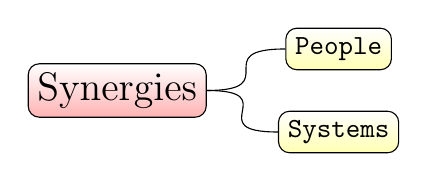
\begin{tikzpicture}
				[grow   = right,
					level distance          = 9em,
					edge from parent path= {(\tikzparentnode.east) .. controls +(1,0) and +(-1,0)  .. (\tikzchildnode.west)},
					every node/.style       = {font=\footnotesize},
					sloped,
					level 1/.style = { level distance = 8em, sibling distance = -3em},
					level 2/.style = {level distance   = 10em, sibling distance = -3em},
				]
				\node [root] {Synergies}
				child { node[syn] {People} }
				child { node[syn] {Systems}}
				;
			\end{tikzpicture}
		\end{column}
		\begin{column}{0.45 \textwidth}
			\begin{itemize}
				\item \textbf{People}: IoT Devices can help all the people. For example, fire detectors, Elders early suppor (by monitoring sounds)
			\end{itemize}
		\end{column}
	\end{columns}
	\begin{itemize}
		\item \textbf{Systems}: Also Devices can be used as input for cloud services, Machine learning,... . Also other Systems
		can be used such as BlockChain or Customer ones.
	\end{itemize}
\end{frame}
